\begin{exampleblock}{Background}
%TODO Put Risk and Utility in smaller font
%TODO Change text about utility and risk sensitivites to a comic
%TODO Change text color of captions
\begin{block}{\normalsize{Risk and Utility}}

Risk: 
\begin{itemize}
    \item Risk is induced by choice with uncertain outcome.
    \item People behave \textbf{risk seeking}, \textbf{risk neutral} or \textbf{risk averse}.
    % \item Risk can exist without the danger of loss (e.g. loosing money).
\end{itemize}

 Utility:
\begin{itemize}
    \item People map money to utility by \textbf{utility function}.
    %\item The same amount of money can have different utility for different people.
    \item Curvature of function defines risk profile.
\end{itemize}


\begin{figure}
  \centering
    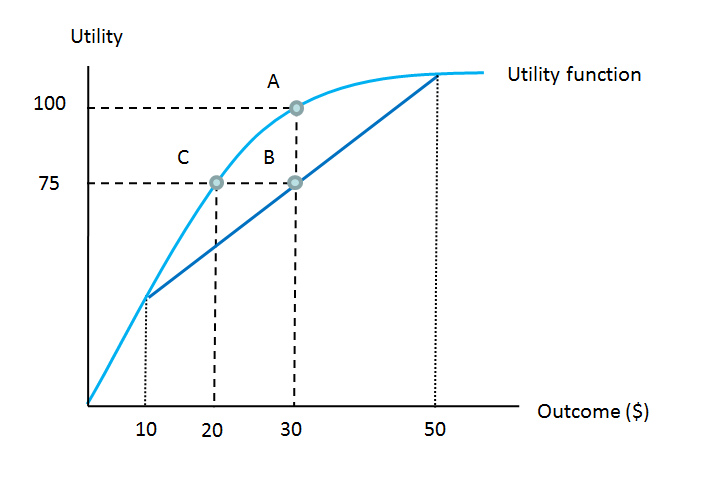
\includegraphics[width=0.9\textwidth]{img/background/riskaversion.jpg}
  \caption{Choice from a lottery where you gain 10\$ or 50\$ by 50\% or a gift of 30\$ for sure. The utility for the fixed reward (point A) is higher than the expected utility of the lottery (point B).}
  
\end{figure}

\end{block}

%TODO Change this block to a plot.
\begin{block}{(Partially Observable) Markov Decision Process}

Making decisions in a partially observable environment.

\begin{itemize}
    \item Set of States $\mathcal{S}$ (Terminal and Non Terminal)
    \item Set of Actions $\mathcal{A}$
    \item Probabilistic Transitions depending on tuple $\mathcal{S} x \mathcal{A}$
    \item Reward function $R(s,a)$
\end{itemize}

For partially observability states are hidden but produce observations:
\begin{itemize}
    \item Observation space $\mathcal{O}$
    \item Observation function $p(o | s, a)$
\end{itemize}

Agent needs to work on probability distribution over all states rather than single deterministic state.
% add reference: http://www.cassandra.org/arc/papers/aaai94.pdf
\end{block}

\end{exampleblock}
